% Compile with pdfLaTeX. Upload main.tex and the images/ folder together.
\documentclass[12pt,a4paper]{article}
\usepackage[utf8]{inputenc}
\usepackage[T5]{fontenc}
\usepackage[english,vietnamese]{babel}
\addto\captionsvietnamese{\renewcommand{\refname}{Tài liệu tham khảo}}
\usepackage[left=2.5cm,right=2cm,top=2.1cm,bottom=2.1cm]{geometry}
\usepackage{amsmath,amssymb,graphicx,booktabs,tabularx,array,longtable}
\usepackage[table]{xcolor}
\usepackage{tikz}
\usetikzlibrary{arrows.meta,positioning,calc,shapes.geometric}
\usepackage{caption,subcaption,enumitem,listings,fancyhdr,titlesec}
\usepackage[protrusion=false]{microtype}
\usepackage{hyperref,xurl}
\hypersetup{unicode=true,colorlinks=true,linkcolor=black,citecolor=blue!45!black,urlcolor=blue!55!black,pdftitle={Bài thực hành 6 - Điều khiển TurtleBot 4 bằng cử chỉ tay},pdfauthor={Sinh viên thực hiện}}
\definecolor{navy}{RGB}{26,57,82}
\definecolor{pale}{RGB}{237,243,247}
\definecolor{codebg}{RGB}{247,248,250}
\linespread{1.10}
\setlength{\parindent}{1em}
\setlength{\parskip}{3pt}
\setlength{\emergencystretch}{2em}
\setlength{\headheight}{15pt}
\setlength{\textfloatsep}{9pt plus 2pt minus 2pt}
\setlength{\intextsep}{8pt plus 2pt minus 2pt}
\setlength{\floatsep}{8pt plus 2pt minus 2pt}
\renewcommand{\topfraction}{0.92}
\renewcommand{\bottomfraction}{0.85}
\renewcommand{\textfraction}{0.07}
\renewcommand{\floatpagefraction}{0.82}
\setcounter{topnumber}{3}
\setcounter{bottomnumber}{3}
\setcounter{totalnumber}{5}
\setcounter{tocdepth}{2}
\setlist{nosep,leftmargin=1.5em,topsep=3pt}
\setlist[itemize]{label=$\bullet$}
\captionsetup{font=small,labelfont=bf,skip=5pt}
\captionsetup[subfigure]{font=small,skip=3pt}
\titleformat{\section}{\large\bfseries\color{navy}}{Chương \thesection.}{0.55em}{}
\titleformat{\subsection}{\normalsize\bfseries}{\thesubsection.}{0.5em}{}
\titlespacing*{\section}{0pt}{13pt}{6pt}
\titlespacing*{\subsection}{0pt}{8pt}{3pt}
\pagestyle{fancy}
\fancyhf{}
\fancyhead[L]{\small Bài thực hành 6 -- TurtleBot 4}
\fancyhead[R]{\small Điều khiển bằng cử chỉ tay}
\fancyfoot[C]{\thepage}
\renewcommand{\headrulewidth}{0.3pt}
\newcolumntype{L}{>{\raggedright\arraybackslash}X}
\newcommand{\code}[1]{\texttt{\detokenize{#1}}}
\newcommand{\smalltable}{\small\setlength{\tabcolsep}{4pt}\renewcommand{\arraystretch}{1.12}}
\lstset{basicstyle=\ttfamily\footnotesize,backgroundcolor=\color{codebg},frame=single,rulecolor=\color{black!20},breaklines=true,breakatwhitespace=false,columns=fullflexible,keepspaces=true,showstringspaces=false,aboveskip=6pt,belowskip=6pt,xleftmargin=3pt,xrightmargin=3pt,tabsize=4}
\tikzset{block/.style={draw=navy,rounded corners=2pt,fill=pale,align=center,font=\small,minimum height=1.0cm,text width=3.3cm},arr/.style={-{Latex[length=2.2mm]},thick,draw=navy},note/.style={font=\scriptsize,align=center,fill=white,inner sep=2pt}}
\raggedbottom
\begin{document}
\hypersetup{pageanchor=false}
\begin{titlepage}
\thispagestyle{empty}
\begin{tikzpicture}[remember picture,overlay]
\draw[navy,line width=0.8pt] ($(current page.north west)+(1.6cm,-1.4cm)$) rectangle ($(current page.south east)+(-1.4cm,1.4cm)$);
\end{tikzpicture}
\centering
{\large\bfseries [TÊN TRƯỜNG / HỌC VIỆN]\\[5pt] [TÊN KHOA / VIỆN]}\par
\vspace{1.5cm}
{\Large\bfseries BÁO CÁO BÀI THỰC HÀNH 6}\par
\vspace{0.7cm}
{\LARGE\bfseries\color{navy} GIAO TIẾP PHI NGÔN NGỮ\\[7pt] VÀ ĐIỀU KHIỂN TURTLEBOT 4\\[7pt] BẰNG CỬ CHỈ TAY}\par
\vspace{0.6cm}
{\large\itshape Non-verbal Human--Robot Interaction\\ Using Hand Gesture Recognition}\par
\vspace{1.6cm}
\begin{tabular}{@{}ll@{}}
Học phần: & [Tên học phần]\\[9pt]
Giảng viên hướng dẫn: & [Họ và tên giảng viên]\\[9pt]
Sinh viên thực hiện: & [Họ và tên sinh viên]\\[9pt]
Mã số sinh viên: & [Mã số sinh viên]\\[9pt]
Lớp / Nhóm: & [Thông tin lớp / nhóm]
\end{tabular}
\vfill
{\large [Địa điểm], tháng [\ldots] năm 2026}\par
\vspace{0.4cm}
\end{titlepage}
\pagenumbering{roman}
\hypersetup{pageanchor=true}
{\setlength{\parskip}{0pt}\renewcommand{\baselinestretch}{0.96}\footnotesize\tableofcontents}
\clearpage
\pagenumbering{arabic}

\section{Giới thiệu bài toán}
\subsection{Mục tiêu và phạm vi}
Bài thực hành xây dựng chuỗi \textbf{webcam $\rightarrow$ nhận diện cử chỉ $\rightarrow$ ROS~2 $\rightarrow$ TurtleBot~4 trong Gazebo}. Hai node ứng dụng sử dụng MediaPipe để nhận năm cử chỉ tĩnh, bổ sung Wave theo chuyển động và điều khiển ba hành vi: chào, bốn chu kỳ tiến--lùi, một vòng tròn. Robot cùng controller nền tảng được tái sử dụng từ các package chính thức~\cite{tb4,source}.
\begin{itemize}
\item \textbf{Chọn--xác nhận:} chọn hành vi chưa làm robot chạy; cần Thumb Up hợp lệ.
\item \textbf{Dừng/hủy:} Open Palm dừng, Closed Fist hủy, mất tín hiệu làm robot dừng.
\item \textbf{Minh chứng:} video webcam thật ngày 24/10/2026, ảnh và odometry; không dùng teleop hoặc cử chỉ giả để lái robot trong demo.
\end{itemize}
Lượt thực nghiệm gồm một người dùng và một video 180,05 giây. Báo cáo đánh giá chức năng của lượt chạy, chưa suy ra độ chính xác trên nhiều người hoặc điều kiện ánh sáng.

\section{Cấu trúc và kiến trúc hệ thống}
\subsection{Sơ đồ kiến trúc tổng thể}
Hình~\ref{fig:architecture} phân biệt hai node chính, đường lệnh và đường phản hồi. OpenCV, MediaPipe, WaveDetector là các thành phần bên trong node nhận diện. Khối Gazebo gộp robot, bridge và controller có sẵn.

\begin{figure}[!htbp]\centering
\resizebox{0.97\linewidth}{!}{\begin{tikzpicture}
\node[block,text width=1.9cm] (cam) at (0,0) {Webcam\\laptop};
\node[block,text width=3.7cm] (rec) at (4.3,0) {\textbf{Node nhận diện}\\{\tiny\ttfamily gesture\_recognition\_node}\\OpenCV + MediaPipe\\Wave theo thời gian};
\node[block,text width=3.9cm] (ctl) at (10.7,0) {\textbf{Node hành vi}\\{\tiny\ttfamily robot\_behavior\_node}\\Chọn--xác nhận\\Kiểm tra và gửi vận tốc};
\node[block,text width=3.7cm] (gui) at (4.3,-3.2) {Cửa sổ webcam\\Nhãn, confidence, landmarks\\Trạng thái robot};
\node[block,text width=3.9cm] (sim) at (10.7,-3.2) {Gazebo + TurtleBot 4\\Vật lý, bridge\\Controller và cảm biến};
\draw[arr] (cam)--node[note,above]{Ảnh BGR}(rec);
\draw[arr] (rec)--node[note,above=11mm]{/detected\_gesture\\std\_msgs/String}(ctl);
\draw[arr] (ctl.north) to[out=100,in=80] node[note,above]{/robot\_behavior\_state}(rec.north);
\draw[arr] (rec)--node[note,right]{Ảnh có chú thích}(gui);
\draw[arr] ($(ctl.south)+(0.8,0)$)--node[note,right]{/cmd\_vel\\TwistStamped}($(sim.north)+(0.8,0)$);
\draw[arr] ($(sim.north)+(-0.8,0)$)--node[note,left]{/odom, /scan, /clock\\dock\_status\\hazard\_detection}($(ctl.south)+(-0.8,0)$);
\end{tikzpicture}}
\caption{Kiến trúc hệ thống: nhận diện, quyết định hành vi và phản hồi mô phỏng.}
\label{fig:architecture}
\end{figure}

\subsection{Cây thư mục và chức năng từng file}
Cây ở Hình~\ref{fig:source-tree} đặt chú thích ngay cạnh file. Package Bài~6 tách riêng với bài SLAM/Nav2/YOLO trước; chỉ tái sử dụng tiện ích môi trường và launch nền tảng.

\begin{figure}[!htbp]\centering
\begin{tikzpicture}[x=1cm,y=0.43cm]
\node[anchor=west,font=\small\bfseries\color{navy}] at (0,1) {CÂY MÃ NGUỒN};
\node[anchor=west,font=\small\bfseries\color{navy}] at (8.2,1) {CHỨC NĂNG};
\draw[black!20] (7.9,1.1)--(7.9,-24.5);
\node[anchor=west,font=\fontsize{8.6}{10}\selectfont] at (0.0,0) {\code{src/turtlebot4_gesture_control/}};
\node[anchor=west,align=left,text width=6.4cm,font=\fontsize{9}{10.5}\selectfont] at (8.2,0) {Package Bài 6; tách khỏi các bài trước.};
\draw[black!40,line width=0.35pt] (0.2,-0.2) |- (0.55,-1);
\node[anchor=west,font=\fontsize{8.6}{10}\selectfont] at (0.65,-1) {\code{turtlebot4_gesture_control/}};
\node[anchor=west,align=left,text width=6.4cm,font=\fontsize{9}{10.5}\selectfont] at (8.2,-1) {Các mô-đun Python.};
\draw[black!40,line width=0.35pt] (0.8500000000000001,-1.2) |- (1.2,-2);
\node[anchor=west,font=\fontsize{8.6}{10}\selectfont] at (1.3,-2) {\code{__init__.py}};
\node[anchor=west,align=left,text width=6.4cm,font=\fontsize{9}{10.5}\selectfont] at (8.2,-2) {Khai báo package Python.};
\draw[black!40,line width=0.35pt] (0.8500000000000001,-1.2) |- (1.2,-3);
\node[anchor=west,font=\fontsize{8.6}{10}\selectfont] at (1.3,-3) {\code{gesture_recognition_node.py}};
\node[anchor=west,align=left,text width=6.4cm,font=\fontsize{9}{10.5}\selectfont] at (8.2,-3) {Webcam, MediaPipe, nhãn và ảnh.};
\draw[black!40,line width=0.35pt] (0.8500000000000001,-1.2) |- (1.2,-4);
\node[anchor=west,font=\fontsize{8.6}{10}\selectfont] at (1.3,-4) {\code{gesture_logic.py}};
\node[anchor=west,align=left,text width=6.4cm,font=\fontsize{9}{10.5}\selectfont] at (8.2,-4) {Wave và máy trạng thái hành vi.};
\draw[black!40,line width=0.35pt] (0.8500000000000001,-1.2) |- (1.2,-5);
\node[anchor=west,font=\fontsize{8.6}{10}\selectfont] at (1.3,-5) {\code{robot_behavior_node.py}};
\node[anchor=west,align=left,text width=6.4cm,font=\fontsize{9}{10.5}\selectfont] at (8.2,-5) {Cảm biến ROS và lệnh vận tốc.};
\draw[black!40,line width=0.35pt] (0.2,-0.2) |- (0.55,-6);
\node[anchor=west,font=\fontsize{8.6}{10}\selectfont] at (0.65,-6) {\code{config/}};
\node[anchor=west,align=left,text width=6.4cm,font=\fontsize{9}{10.5}\selectfont] at (8.2,-6) {Thông số vận hành.};
\draw[black!40,line width=0.35pt] (0.8500000000000001,-6.2) |- (1.2,-7);
\node[anchor=west,font=\fontsize{8.6}{10}\selectfont] at (1.3,-7) {\code{behavior.yaml}};
\node[anchor=west,align=left,text width=6.4cm,font=\fontsize{9}{10.5}\selectfont] at (8.2,-7) {Tốc độ, quãng đường và timeout.};
\draw[black!40,line width=0.35pt] (0.2,-0.2) |- (0.55,-8);
\node[anchor=west,font=\fontsize{8.6}{10}\selectfont] at (0.65,-8) {\code{launch/}};
\node[anchor=west,align=left,text width=6.4cm,font=\fontsize{9}{10.5}\selectfont] at (8.2,-8) {Các lệnh khởi chạy.};
\draw[black!40,line width=0.35pt] (0.8500000000000001,-8.2) |- (1.2,-9);
\node[anchor=west,font=\fontsize{8.6}{10}\selectfont] at (1.3,-9) {\code{arena.launch.py}};
\node[anchor=west,align=left,text width=6.4cm,font=\fontsize{9}{10.5}\selectfont] at (8.2,-9) {Mô phỏng; robot giữa sân, dock ở góc.};
\draw[black!40,line width=0.35pt] (0.8500000000000001,-8.2) |- (1.2,-10);
\node[anchor=west,font=\fontsize{8.6}{10}\selectfont] at (1.3,-10) {\code{behavior.launch.py}};
\node[anchor=west,align=left,text width=6.4cm,font=\fontsize{9}{10.5}\selectfont] at (8.2,-10) {Nạp YAML và chạy node hành vi.};
\draw[black!40,line width=0.35pt] (0.8500000000000001,-8.2) |- (1.2,-11);
\node[anchor=west,font=\fontsize{8.6}{10}\selectfont] at (1.3,-11) {\code{gui.launch.py}};
\node[anchor=west,align=left,text width=6.4cm,font=\fontsize{9}{10.5}\selectfont] at (8.2,-11) {Mở lại GUI, giữ server đang chạy.};
\draw[black!40,line width=0.35pt] (0.2,-0.2) |- (0.55,-12);
\node[anchor=west,font=\fontsize{8.6}{10}\selectfont] at (0.65,-12) {\code{worlds/}};
\node[anchor=west,align=left,text width=6.4cm,font=\fontsize{9}{10.5}\selectfont] at (8.2,-12) {Tài nguyên môi trường.};
\draw[black!40,line width=0.35pt] (0.8500000000000001,-12.2) |- (1.2,-13);
\node[anchor=west,font=\fontsize{8.6}{10}\selectfont] at (1.3,-13) {\code{gesture_arena.sdf}};
\node[anchor=west,align=left,text width=6.4cm,font=\fontsize{9}{10.5}\selectfont] at (8.2,-13) {Sân 16 x 16 m, sàn và tường bao.};
\draw[black!40,line width=0.35pt] (0.2,-0.2) |- (0.55,-14);
\node[anchor=west,font=\fontsize{8.6}{10}\selectfont] at (0.65,-14) {\code{scripts/}};
\node[anchor=west,align=left,text width=6.4cm,font=\fontsize{9}{10.5}\selectfont] at (8.2,-14) {Chuẩn bị phụ thuộc.};
\draw[black!40,line width=0.35pt] (0.8500000000000001,-14.2) |- (1.2,-15);
\node[anchor=west,font=\fontsize{8.6}{10}\selectfont] at (1.3,-15) {\code{setup_gesture.sh}};
\node[anchor=west,align=left,text width=6.4cm,font=\fontsize{9}{10.5}\selectfont] at (8.2,-15) {Tạo venv và tải model MediaPipe.};
\draw[black!40,line width=0.35pt] (0.2,-0.2) |- (0.55,-16);
\node[anchor=west,font=\fontsize{8.6}{10}\selectfont] at (0.65,-16) {\code{test/}};
\node[anchor=west,align=left,text width=6.4cm,font=\fontsize{9}{10.5}\selectfont] at (8.2,-16) {Kiểm thử logic và launch.};
\draw[black!40,line width=0.35pt] (0.8500000000000001,-16.2) |- (1.2,-17);
\node[anchor=west,font=\fontsize{8.6}{10}\selectfont] at (1.3,-17) {\code{test_gesture_logic.py}};
\node[anchor=west,align=left,text width=6.4cm,font=\fontsize{9}{10.5}\selectfont] at (8.2,-17) {Xác nhận, dừng, Wave, tiến độ.};
\draw[black!40,line width=0.35pt] (0.8500000000000001,-16.2) |- (1.2,-18);
\node[anchor=west,font=\fontsize{8.6}{10}\selectfont] at (1.3,-18) {\code{test_arena_world.py}};
\node[anchor=west,align=left,text width=6.4cm,font=\fontsize{9}{10.5}\selectfont] at (8.2,-18) {World bridge và vị trí dock/TF.};
\draw[black!40,line width=0.35pt] (0.2,-0.2) |- (0.55,-19);
\node[anchor=west,font=\fontsize{8.6}{10}\selectfont] at (0.65,-19) {\code{resource/}};
\node[anchor=west,align=left,text width=6.4cm,font=\fontsize{9}{10.5}\selectfont] at (8.2,-19) {Đăng ký package với ament.};
\draw[black!40,line width=0.35pt] (0.2,-0.2) |- (0.55,-20);
\node[anchor=west,font=\fontsize{8.6}{10}\selectfont] at (0.65,-20) {\code{setup.py}};
\node[anchor=west,align=left,text width=6.4cm,font=\fontsize{9}{10.5}\selectfont] at (8.2,-20) {Executable và tài nguyên cài đặt.};
\draw[black!40,line width=0.35pt] (0.2,-0.2) |- (0.55,-21);
\node[anchor=west,font=\fontsize{8.6}{10}\selectfont] at (0.65,-21) {\code{setup.cfg}};
\node[anchor=west,align=left,text width=6.4cm,font=\fontsize{9}{10.5}\selectfont] at (8.2,-21) {Vị trí cài các executable Python.};
\draw[black!40,line width=0.35pt] (0.2,-0.2) |- (0.55,-22);
\node[anchor=west,font=\fontsize{8.6}{10}\selectfont] at (0.65,-22) {\code{package.xml}};
\node[anchor=west,align=left,text width=6.4cm,font=\fontsize{9}{10.5}\selectfont] at (8.2,-22) {Tên package, phụ thuộc, kiểu build.};
\draw[black!40,line width=0.35pt] (0.2,-0.2) |- (0.55,-23);
\node[anchor=west,font=\fontsize{8.6}{10}\selectfont] at (0.65,-23) {\code{README.md}};
\node[anchor=west,align=left,text width=6.4cm,font=\fontsize{9}{10.5}\selectfont] at (8.2,-23) {Câu lệnh và quy trình demo.};
\draw[black!40,line width=0.35pt] (0.2,-0.2) |- (0.55,-24);
\node[anchor=west,font=\fontsize{8.6}{10}\selectfont] at (0.65,-24) {\code{VALIDATION.md}};
\node[anchor=west,align=left,text width=6.4cm,font=\fontsize{9}{10.5}\selectfont] at (8.2,-24) {Kết quả và giới hạn kiểm thử.};
\end{tikzpicture}
\caption{Cây thư mục package với chức năng ngắn gọn đặt ngay cạnh từng file.}
\label{fig:source-tree}
\end{figure}

\subsection{Node, topic và dữ liệu trao đổi}
ROS~2 hỗ trợ một node đồng thời publish và subscribe nhiều topic~\cite{ros_topics}. Vai trò hai node ứng dụng được tóm tắt như sau:

\begin{table}[!htbp]\centering\smalltable
\begin{tabularx}{\linewidth}{@{}p{4.3cm}LL@{}}\toprule
\textbf{Node} & \textbf{Đầu vào} & \textbf{Xử lý / đầu ra}\\\midrule
\path{gesture_recognition_node} & Webcam; trạng thái hành vi. & Nhận diện, lọc, hiển thị; publish nhãn, ảnh và debug.\\
\path{robot_behavior_node} & Cử chỉ; odom, scan, clock, dock, bumper. & Quản lý trạng thái; publish vận tốc và trạng thái.\\\bottomrule
\end{tabularx}
\caption{Hai node chính trong chuỗi điều khiển.}
\end{table}

Trong lượt quay còn có node quan sát \path{lab06_demo_observer} để lưu sự kiện/odom và nhắc bước. Node này chỉ subscribe, không gửi cử chỉ hay vận tốc.

\begin{table}[!htbp]\centering\smalltable
\begin{tabularx}{\linewidth}{@{}p{4.8cm}p{5.1cm}L@{}}\toprule
\textbf{Topic} & \textbf{Kiểu message} & \textbf{Vai trò}\\\midrule
\path{/detected_gesture} & \path{std_msgs/msg/String} & Nhãn hoặc None.\\
\path{/cmd_vel} & \shortstack[l]{\code{geometry_msgs/msg/}\\\code{TwistStamped}} & Vận tốc và timestamp.\\
\path{/odom} & \path{nav_msgs/msg/Odometry} & Tiến độ vị trí/góc.\\
\path{/scan} & \shortstack[l]{\code{sensor_msgs/msg/}\\\code{LaserScan}} & Khoảng đo vật cản.\\
\path{/clock} & \path{rosgraph_msgs/msg/Clock} & Đồng hồ mô phỏng.\\
\path{/dock_status} & \shortstack[l]{\code{irobot_create_msgs/msg/}\\\code{DockStatus}} & Robot có ở dock hay không.\\
\path{/hazard_detection} & \shortstack[l]{\code{irobot_create_msgs/msg/}\\\code{HazardDetectionVector}} & Phản hồi bumper.\\
\path{/robot_behavior_state} & \path{std_msgs/msg/String} & JSON trạng thái và ready.\\
\shortstack[l]{\code{/gesture_recognition}\\\code{/image}} & \path{sensor_msgs/msg/Image} & Ảnh đã chú thích.\\
\shortstack[l]{\code{/gesture_recognition}\\\code{/debug}} & \path{std_msgs/msg/String} & Nhãn gốc, confidence, thời gian xử lý.\\\bottomrule
\end{tabularx}
\caption{Giao diện topic của bản triển khai ROS~2 Jazzy.}
\label{tab:topics}
\end{table}

\path{/cmd_vel} dùng \code{TwistStamped}, gồm header và twist~\cite{twist}; lệnh sử dụng \code{linear.x}, \code{angular.z}, timestamp mô phỏng và frame \code{base_link}. Trạng thái có QoS transient local; các cảm biến dùng QoS sensor data.

\section{Nhận diện cử chỉ tay}
\subsection{Luồng xử lý ảnh}

\begin{figure}[!htbp]\centering
\resizebox{\linewidth}{!}{\begin{tikzpicture}
\node[block,text width=2.2cm] (a) at (0,0) {Webcam\\640 $\times$ 480};
\node[block,text width=2.2cm] (b) at (3.1,0) {Lật gương\\BGR $\rightarrow$ RGB};
\node[block,text width=2.6cm] (c) at (6.5,0) {MediaPipe VIDEO\\Nhãn + 21 landmarks};
\node[block,text width=2.5cm] (d) at (10.0,0) {Lọc confidence\\Phân biệt Wave};
\node[block,text width=2.5cm] (e) at (13.5,0) {Publish nhãn\\Vẽ và hiển thị ảnh};
\foreach \s/\t in {a/b,b/c,c/d,d/e}\draw[arr](\s)--(\t);
\node[draw=red!50!black,fill=red!4,rounded corners,align=center,font=\small] (none) at (10,-1.9) {Không đủ tin cậy / ảnh cũ\\$\rightarrow$ publish \texttt{None}};
\draw[arr,draw=red!60!black](d)--(none);
\end{tikzpicture}}
\caption{Luồng nhận diện. Kết quả không hợp lệ không được giữ làm lệnh cũ.}
\label{fig:vision-flow}
\end{figure}

OpenCV đọc webcam bằng \code{VideoCapture}~\cite{opencv}. Model \path{gesture_recognizer.task} chạy chế độ \code{VIDEO}, một bàn tay, timestamp tăng nghiêm ngặt và lời gọi \code{recognize_for_video}~\cite{mp_python}. Capture/suy luận nằm ở một luồng riêng; timer ROS chỉ lấy kết quả gần nhất để tránh hàng đợi ảnh cũ.

\begin{table}[!htbp]\centering\smalltable
\begin{tabularx}{\linewidth}{@{}p{4.5cm}p{2.5cm}L@{}}\toprule
\textbf{Điều kiện} & \textbf{Cấu hình} & \textbf{Tác dụng}\\\midrule
Confidence phân loại & $\geq0{,}65$ & Loại kết quả không đủ tin cậy.\\
Tuổi ảnh tối đa & 0,35 s & Ảnh cũ tạo None.\\
Publish kết quả & 10 Hz & Nhịp gửi tín hiệu điều khiển.\\
Giới hạn capture & 15 fps & Giới hạn vòng đọc/xử lý, không phải FPS đã đo.\\\bottomrule
\end{tabularx}
\caption{Các điều kiện xử lý ở node nhận diện.}
\end{table}

Landmarks còn xuất hiện chưa chắc nhãn đã hợp lệ. Năm nhãn tĩnh dùng trong bài là Pointing Up, Victory, Thumb Up, Open Palm và Closed Fist~\cite{mp_overview}; các nhãn khác hoặc không đủ điều kiện đều tạo None.

\subsection{Phân biệt Wave với Open Palm}
Wave không phải nhãn dựng sẵn của model. Hệ thống kết hợp Open Palm với chuyển động trung bình của bốn đầu ngón:
\begin{equation}
 x_h=\frac{x_8+x_{12}+x_{16}+x_{20}}{4},\qquad
 A=\max(x_h)-\min(x_h).
\end{equation}

\begin{figure}[!htbp]\centering
\resizebox{0.98\linewidth}{!}{\begin{tikzpicture}
\node[block,text width=2.4cm] (a) at (0,0) {AI nhận\\Open Palm};
\node[block,text width=2.8cm] (b) at (3.7,0) {Theo dõi $x_h$\\trong 3 giây};
\node[block,text width=3.3cm] (c) at (8.0,0) {$A\geq0{,}09$ chiều rộng ảnh\\$\geq2$ lần đảo chiều\\Hysteresis: 0,025};
\node[block,text width=2.4cm] (d) at (12.2,0) {Còn chuyển động\\$\rightarrow$ Wave};
\draw[arr](a)--(b);\draw[arr](b)--(c);\draw[arr](c)--(d);
\node[draw=navy,fill=pale,rounded corners,align=center,font=\small] (p) at (6.1,-2) {Đứng yên $>0{,}25$ s: xóa lịch sử Wave $\rightarrow$ Open Palm};
\draw[arr](b.south)--(b.south|-p.north);\draw[arr](d.south)--(d.south|-p.north);
\end{tikzpicture}}
\caption{Wave là cử chỉ động; bàn tay mở đứng yên vẫn là lệnh dừng.}
\label{fig:wave-flow}
\end{figure}

Một lần quét ngang chưa đủ thành Wave. Lịch sử được làm mới khi đổi tay, mất mẫu lâu hoặc vị trí nhảy bất thường; một frame không chắc chắn vẫn publish None. Điểm hiển thị của Wave là confidence Open Palm kết hợp điều kiện chuyển động, không phải điểm của một mô hình Wave huấn luyện riêng.

\section{Điều khiển hành vi robot}
\subsection{Bảng ánh xạ cử chỉ}

\begin{table}[!htbp]\centering\smalltable
\begin{tabularx}{\linewidth}{@{}p{3cm}Lp{4.3cm}@{}}\toprule
\textbf{Cử chỉ} & \textbf{Hành vi} & \textbf{Điều kiện}\\\midrule
Wave & Chọn quay chào trái--phải. & Chờ Thumb Up.\\
Pointing Up & Chọn bốn chu kỳ tiến--lùi. & Chờ Thumb Up.\\
Victory & Chọn đi một vòng tròn. & Chờ Thumb Up.\\
Thumb Up & Xác nhận hành vi đã chọn. & Robot đủ điều kiện chạy.\\
Open Palm & Dừng, xóa lựa chọn. & Không chờ xác nhận.\\
Closed Fist & Hủy, trở về chờ. & Không chờ xác nhận.\\\bottomrule
\end{tabularx}
\caption{Ánh xạ sáu cử chỉ với hành vi TurtleBot~4.}
\label{tab:mapping}
\end{table}

\subsection{Máy trạng thái chọn--xác nhận}

\begin{figure}[!htbp]\centering
\resizebox{\linewidth}{!}{\begin{tikzpicture}
\node[block,text width=2.7cm] (idle) at (0,0) {Chờ\\\texttt{IDLE}};
\node[block,text width=2.7cm] (sel) at (4,0) {Đã chọn\\\texttt{SELECTED}};
\node[block,text width=2.7cm] (run) at (8,0) {Đang chạy\\\texttt{RUNNING}};
\node[block,text width=2.7cm] (done) at (12,0) {Hoàn thành\\\texttt{COMPLETED}};
\draw[arr](idle)--node[note,above=6mm]{Cử chỉ chọn\\ổn định}(sel);
\draw[arr](sel)--node[note,above=6mm]{Thumb Up\\và ready}(run);
\draw[arr](run)--node[note,above=6mm]{Đủ tiến độ\\theo odom}(done);
\draw[arr](done.north)to[out=110,in=70]node[note,above]{Chọn mới}(sel.north);
\node[block,text width=13.2cm,draw=red!50!black,fill=red!4] (stop) at (6,-2.4) {\textbf{Ngắt và xóa lựa chọn}\\Open Palm $\rightarrow$ STOPPED; Closed Fist $\rightarrow$ IDLE;\\mất cử chỉ $\rightarrow$ SIGNAL\_LOST; lỗi cảm biến khi chạy $\rightarrow$ SAFETY\_STOP.};
\draw[arr,draw=red!60!black](run.south)--(run.south|-stop.north);
\draw[arr,draw=red!60!black](sel.south)--(sel.south|-stop.north);
\end{tikzpicture}}
\caption{Luồng trạng thái chính. Chọn/xác nhận bị lọc theo thời gian; dừng/hủy được ưu tiên.}
\label{fig:states}
\end{figure}

\begin{itemize}
\item Chọn và xác nhận phải ổn định 0,35 s; lựa chọn hết hạn sau 10 s.
\item Giữ một cử chỉ không phát lệnh lặp liên tục. Trong RUNNING, cử chỉ chọn mới không thay hành vi hiện tại.
\item Hoàn thành hoặc bị ngắt đều xóa lựa chọn. Xác nhận khi thiếu dữ liệu tạo NOT\_READY.
\item Vận hành bằng cách giữ Thumb Up trong khung hình; heartbeat từ cử chỉ hợp lệ duy trì điều khiển, nhưng Open Palm/Closed Fist luôn dừng/hủy.
\end{itemize}

\subsection{Quỹ đạo và phản hồi odometry}

\begin{table}[!htbp]\centering\smalltable
\begin{tabularx}{\linewidth}{@{}p{2.5cm}Lp{4.5cm}@{}}\toprule
\textbf{Hành vi} & \textbf{Lệnh và chuỗi pha} & \textbf{Điều kiện hoàn thành}\\\midrule
Tiến--lùi & Tám lượt luân phiên; mỗi lượt 0,35 m; $v=\pm0{,}24$ m/s. & Mỗi pha đạt tổng dịch chuyển mục tiêu.\\
Vòng tròn & $R=0{,}60$ m; $v=0{,}24$ m/s; $\omega=v/R=0{,}40$ rad/s. & $\sum|\Delta\theta|\geq2\pi$.\\
Chào & Góc pha $+0{,}45$, $-0{,}90$, $+0{,}45$ rad; $|\omega|=0{,}90$ rad/s. & Đạt tiến độ từng pha quay.\\\bottomrule
\end{tabularx}
\caption{Ba chuyển động được thực hiện theo phản hồi, không chỉ bằng thời gian chờ cố định.}
\end{table}

Tiến độ dùng $\Delta s=\sqrt{\Delta x^2+\Delta y^2}$ hoặc biến thiên yaw đã chuẩn hóa. Controller còn tăng/giảm tốc nên vị trí thực có thể vượt ngưỡng sau khi chuyển pha; triển khai hiện tại chưa điều khiển vị trí theo sai số có dấu.

\subsection{Điều kiện chạy và xử lý dừng}

\begin{table}[!htbp]\centering\smalltable
\begin{tabularx}{\linewidth}{@{}p{4.6cm}p{3.7cm}L@{}}\toprule
\textbf{Điều kiện} & \textbf{Ngưỡng / trạng thái} & \textbf{Xử lý}\\\midrule
Cử chỉ chọn/xác nhận & Ổn định 0,35 s & Chấp nhận một sự kiện.\\
Thiếu cử chỉ hợp lệ & Quá 0,65 s & SIGNAL\_LOST, vận tốc về 0.\\
Odom/scan không còn mới & Quá 0,80 s & Không cho bắt đầu; đang chạy thì dừng.\\
Robot docked / có bumper & ready không đạt & Chặn chạy hoặc SAFETY\_STOP.\\
Khoảng đo LiDAR nhỏ & Dưới 0,35 m theo hướng chạy & OBSTACLE\_STOP.\\
Hành vi quá lâu & Quá 180 s thực & TIMEOUT.\\\bottomrule
\end{tabularx}
\caption{Các lớp bảo vệ trong điều khiển.}
\end{table}

Timer hành vi 20~Hz và watchdog dùng đồng hồ steady; timestamp lệnh dùng thời gian mô phỏng. Ready còn yêu cầu scan hợp lệ trước/sau và clock đã bắt đầu. Kiểm tra LiDAR là điều kiện dừng, không phải bộ lập kế hoạch tránh vật cản; sân demo được để trống, dock đặt ở góc $(6,6)$.

\section{Triển khai và vận hành}
\subsection{Môi trường thực hiện}

\begin{table}[!htbp]\centering\smalltable
\begin{tabularx}{\linewidth}{@{}p{4.2cm}L@{}}\toprule
\textbf{Thành phần} & \textbf{Cấu hình}\\\midrule
Nền tảng & Ubuntu 24.04, ROS~2 Jazzy, Python 3.12.\\
Mô phỏng & Gazebo Harmonic, TurtleBot~4 Standard, sân 16 $\times$ 16 m.\\
Nhận diện & MediaPipe 0.10.21, OpenCV 4.6.0, NumPy 1.26.4; venv riêng.\\
Giao tiếp & Cùng ROS domain 76 và Gazebo partition tương ứng.\\
Ghi hình & MP4 H.264, 1920 $\times$ 1080, 20 fps; không âm thanh.\\\bottomrule
\end{tabularx}
\caption{Môi trường dùng trong lượt thực nghiệm.}
\end{table}

\subsection{Câu lệnh khởi chạy}
Nạp môi trường dưới đây trong \textbf{mỗi terminal}; build và cài model chỉ cần thực hiện khi chuẩn bị dự án:
\begin{lstlisting}[language=bash]
cd ~/tb4_ws
export TB4_LAB_DOMAIN_ID=76
source src/turtlebot4_slam_nav/scripts/env.sh
export GZ_IP=127.0.0.1

# Build/setup when preparing the project
colcon build --symlink-install \
  --packages-up-to turtlebot4_gesture_control
source install/local_setup.bash
bash src/turtlebot4_gesture_control/scripts/setup_gesture.sh
\end{lstlisting}
\begin{lstlisting}[language=bash,caption={Ba lệnh vận hành chạy trong ba terminal đã nạp môi trường.}]
# Terminal A: Gazebo
ros2 launch turtlebot4_gesture_control arena.launch.py \
  gui_render_engine:=ogre

# Terminal B: behavior
ros2 launch turtlebot4_gesture_control behavior.launch.py

# Terminal C: perception
./.venv-gesture/bin/python -m \
  turtlebot4_gesture_control.gesture_recognition_node \
  --ros-args -p camera_index:=0 -p confidence:=0.65 \
  -p max_fps:=15.0
\end{lstlisting}
Chờ \code{ready=True}, chọn cử chỉ rồi Thumb Up xác nhận; giữ tay được nhận diện khi robot chạy. Sửa YAML cần chạy lại node hành vi. Robot xuất phát ngoài dock trong sân mặc định nên không cần Undock.

\subsection{Kiểm tra trước demo và khôi phục GUI}
\begin{lstlisting}[language=bash]
ros2 topic type /cmd_vel
ros2 topic hz /scan
ros2 topic hz /odom
ros2 topic echo /detected_gesture
ros2 topic echo /robot_behavior_state \
  --qos-durability transient_local
\end{lstlisting}
Các lệnh theo dõi chạy riêng, dừng bằng Ctrl+C khi chuyển lệnh. GUI dùng Ogre1, server/LiDAR dùng Ogre2. Mở lại GUI trong terminal cùng domain bằng lệnh sau; nếu server đã dừng, chạy lại arena.
\begin{lstlisting}[language=bash]
ros2 launch turtlebot4_gesture_control gui.launch.py
\end{lstlisting}

\section{Kết quả thực nghiệm và đánh giá}
\subsection{Dữ liệu và kịch bản}
Bộ minh chứng~\cite{experiment} gồm video 180,05 giây ngày 24/10/2026, ảnh, log trạng thái và odometry. Người dùng làm cử chỉ thật; công cụ ghi chỉ quan sát topic. Thứ tự cảnh: tiến--lùi, vòng tròn, chào, dừng bằng Open Palm, hủy bằng Closed Fist và mất tín hiệu.

\begin{figure}[!htbp]\centering
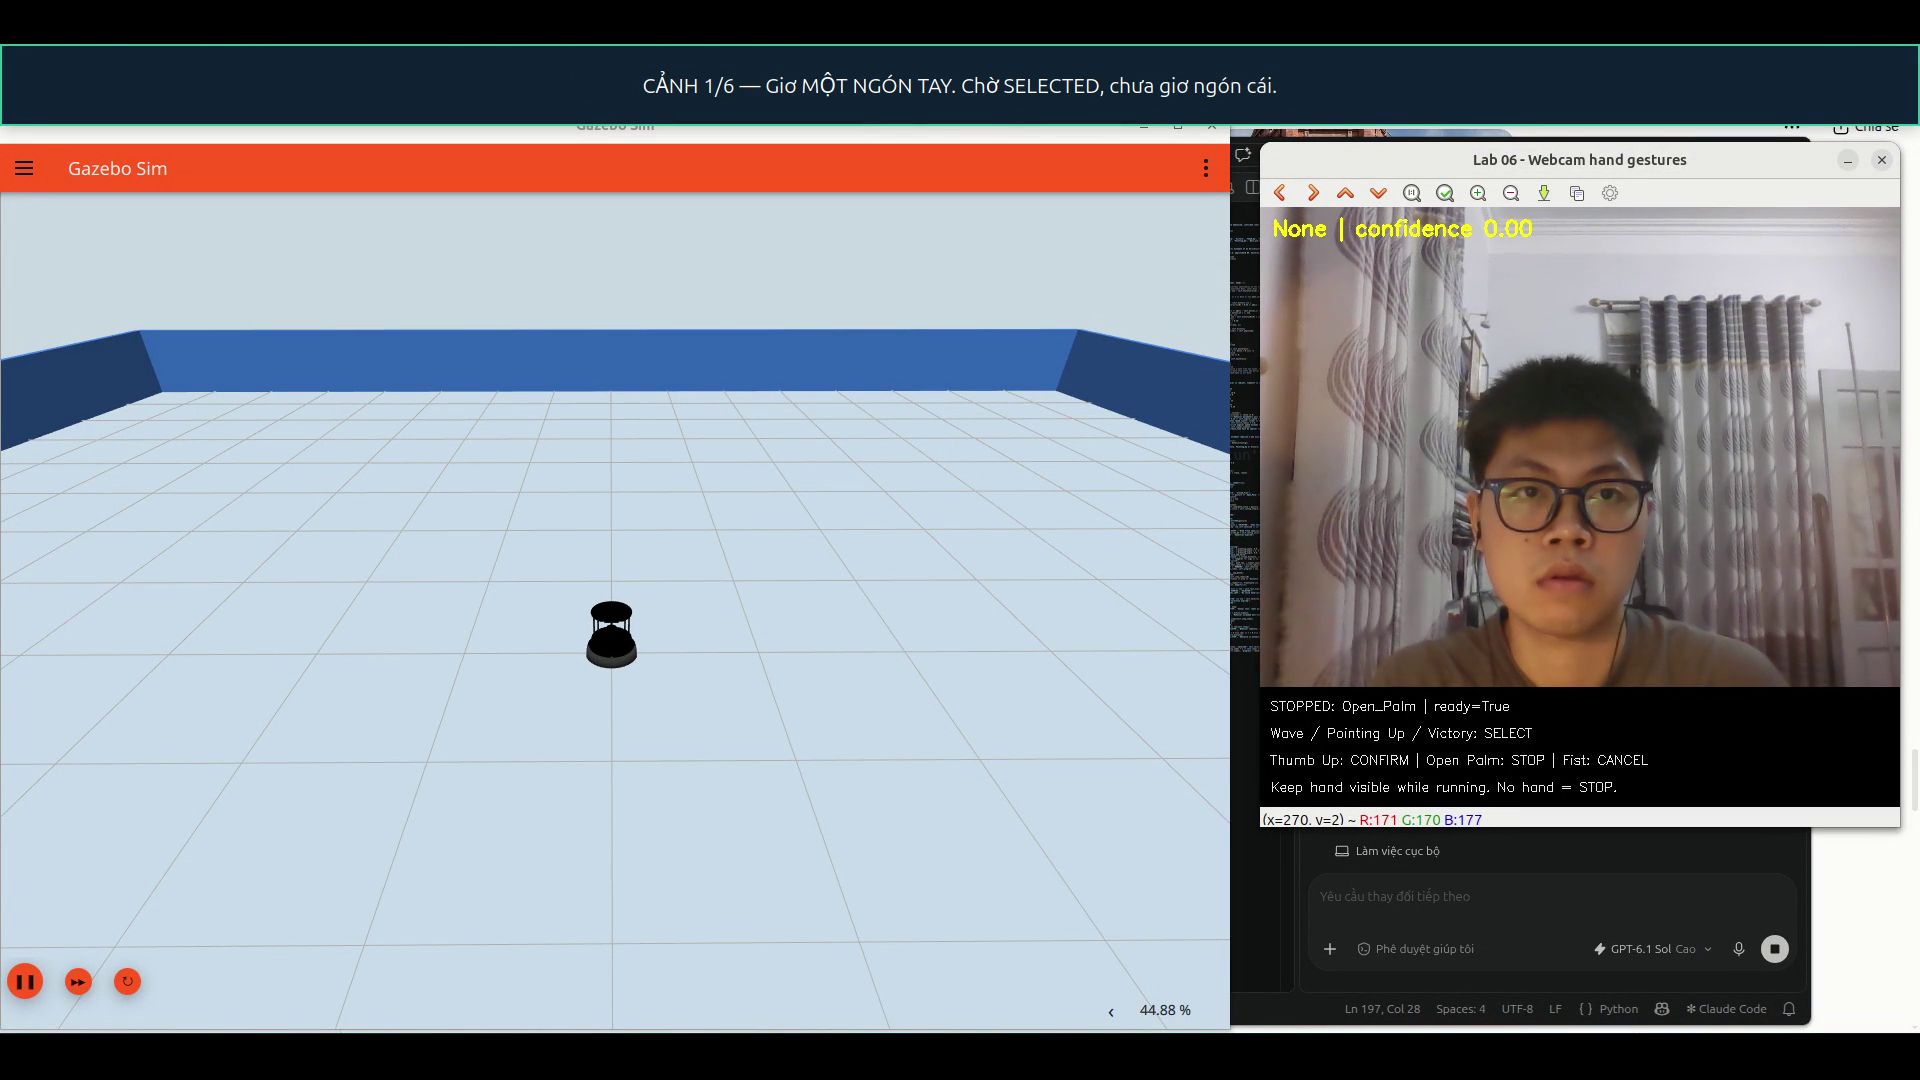
\includegraphics[width=0.78\linewidth]{images/01_ready_overview.png}
\caption{Bố trí ghi hình đồng thời Gazebo, webcam và thanh hướng dẫn.}
\label{fig:overview}
\end{figure}

\subsection{Minh họa sáu cử chỉ}

\begin{figure}[!htbp]\centering
\begin{subfigure}{0.32\linewidth}\centering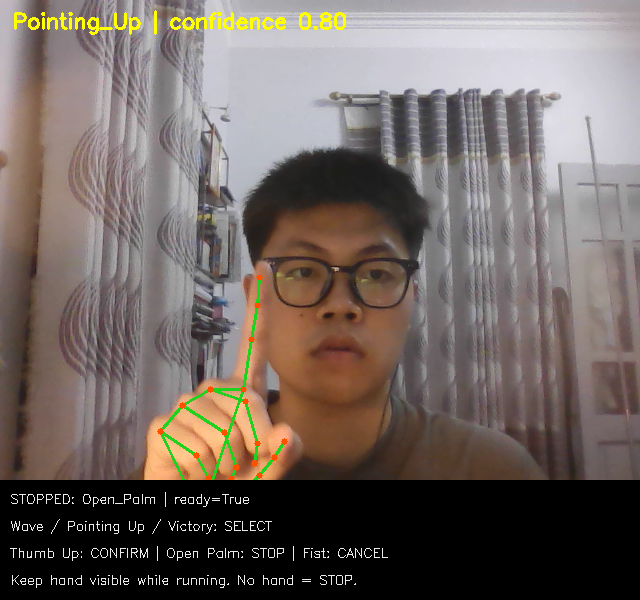
\includegraphics[width=\linewidth,trim=0bp 120bp 0bp 0bp,clip]{images/gesture_Pointing_Up.png}\caption{Pointing Up}\end{subfigure}\hfill
\begin{subfigure}{0.32\linewidth}\centering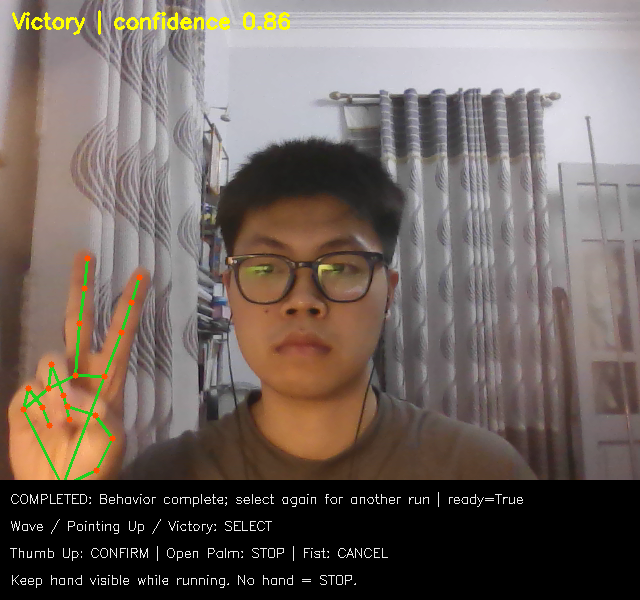
\includegraphics[width=\linewidth,trim=0bp 120bp 0bp 0bp,clip]{images/gesture_Victory.png}\caption{Victory}\end{subfigure}\hfill
\begin{subfigure}{0.32\linewidth}\centering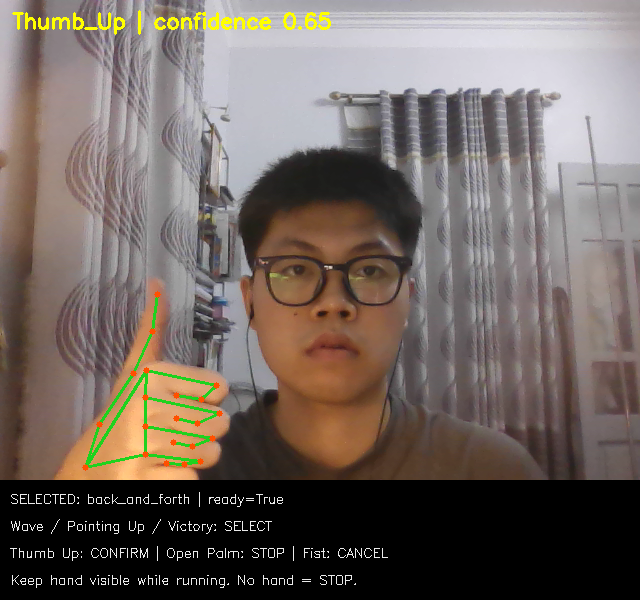
\includegraphics[width=\linewidth,trim=0bp 120bp 0bp 0bp,clip]{images/gesture_Thumb_Up.png}\caption{Thumb Up}\end{subfigure}
\par\smallskip
\begin{subfigure}{0.32\linewidth}\centering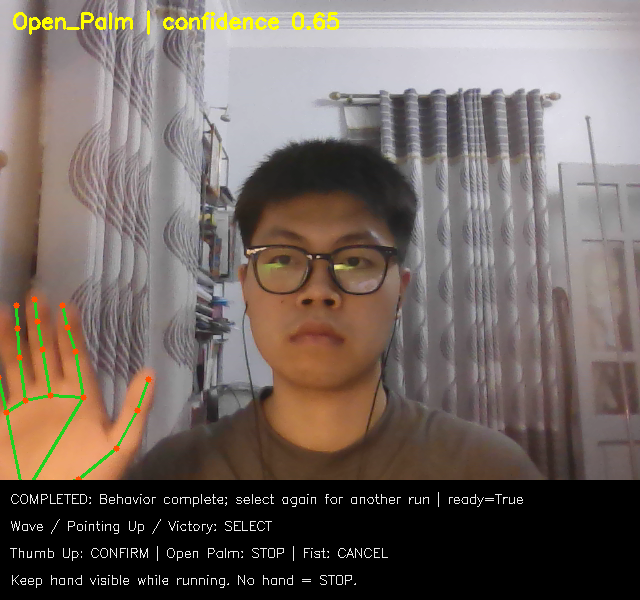
\includegraphics[width=\linewidth,trim=0bp 120bp 0bp 0bp,clip]{images/gesture_Open_Palm.png}\caption{Open Palm}\end{subfigure}\hfill
\begin{subfigure}{0.32\linewidth}\centering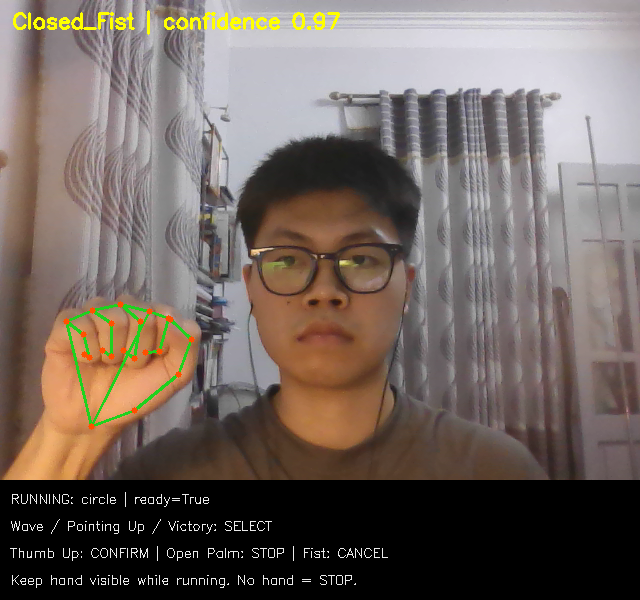
\includegraphics[width=\linewidth,trim=0bp 120bp 0bp 0bp,clip]{images/gesture_Closed_Fist.png}\caption{Closed Fist}\end{subfigure}\hfill
\begin{subfigure}{0.32\linewidth}\centering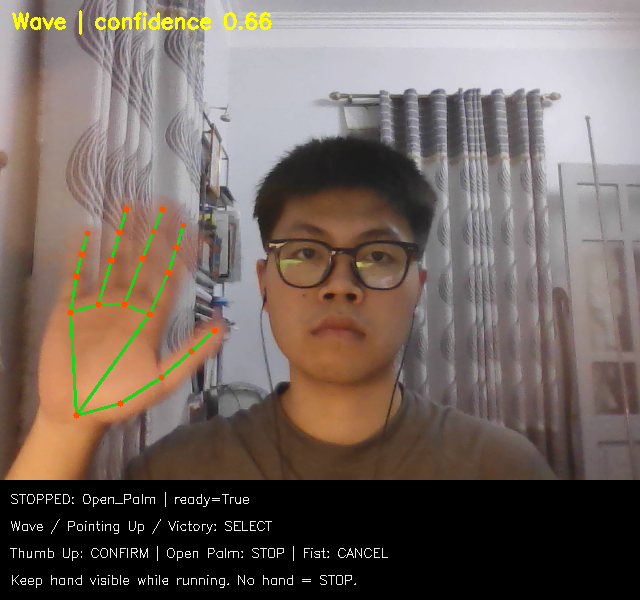
\includegraphics[width=\linewidth,trim=0bp 120bp 0bp 0bp,clip]{images/gesture_Wave.png}\caption{Wave}\end{subfigure}
\caption{Ảnh thật trong lượt quay; chỉ lược phần hướng dẫn phía dưới khi dàn trang. Một ảnh Wave minh họa nhãn, còn điều kiện chuyển động được đối chiếu bằng video.}
\label{fig:sixgestures}
\end{figure}

\begin{table}[!htbp]\centering\smalltable
\begin{tabularx}{\linewidth}{@{}p{3.4cm}p{2.5cm}L@{}}\toprule
\textbf{Nhãn} & \textbf{Confidence mẫu} & \textbf{Lưu ý}\\\midrule
Pointing Up & 0,7967 & Mẫu một ngón.\\
Victory & 0,8582 & Mẫu hai ngón.\\
Thumb Up & 0,6525 & Gần ngưỡng 0,65.\\
Open Palm & 0,6534 & Tay gần biên ảnh.\\
Closed Fist & 0,9742 & Mẫu nắm tay.\\
Wave & 0,6595 & Điểm Open Palm cộng điều kiện động.\\\bottomrule
\end{tabularx}
\caption{Điểm của ảnh mẫu đầu tiên nhận được ở mỗi nhãn, không phải điểm trung bình hay tỷ lệ chính xác.}
\end{table}

\subsection{Kết quả chuyển động và xác nhận}
Ở cảnh đầu, robot vẫn đứng yên khi Pointing Up đã tạo SELECTED; chỉ sau Thumb Up mới chuyển RUNNING. Log ghi đủ tám pha tiến/lùi. Hình~\ref{fig:motion-overview} gộp dữ liệu của ba hành vi thành công để đối chiếu số chu kỳ, hình dạng quỹ đạo và thứ tự quay.

\begin{figure}[!htbp]\centering
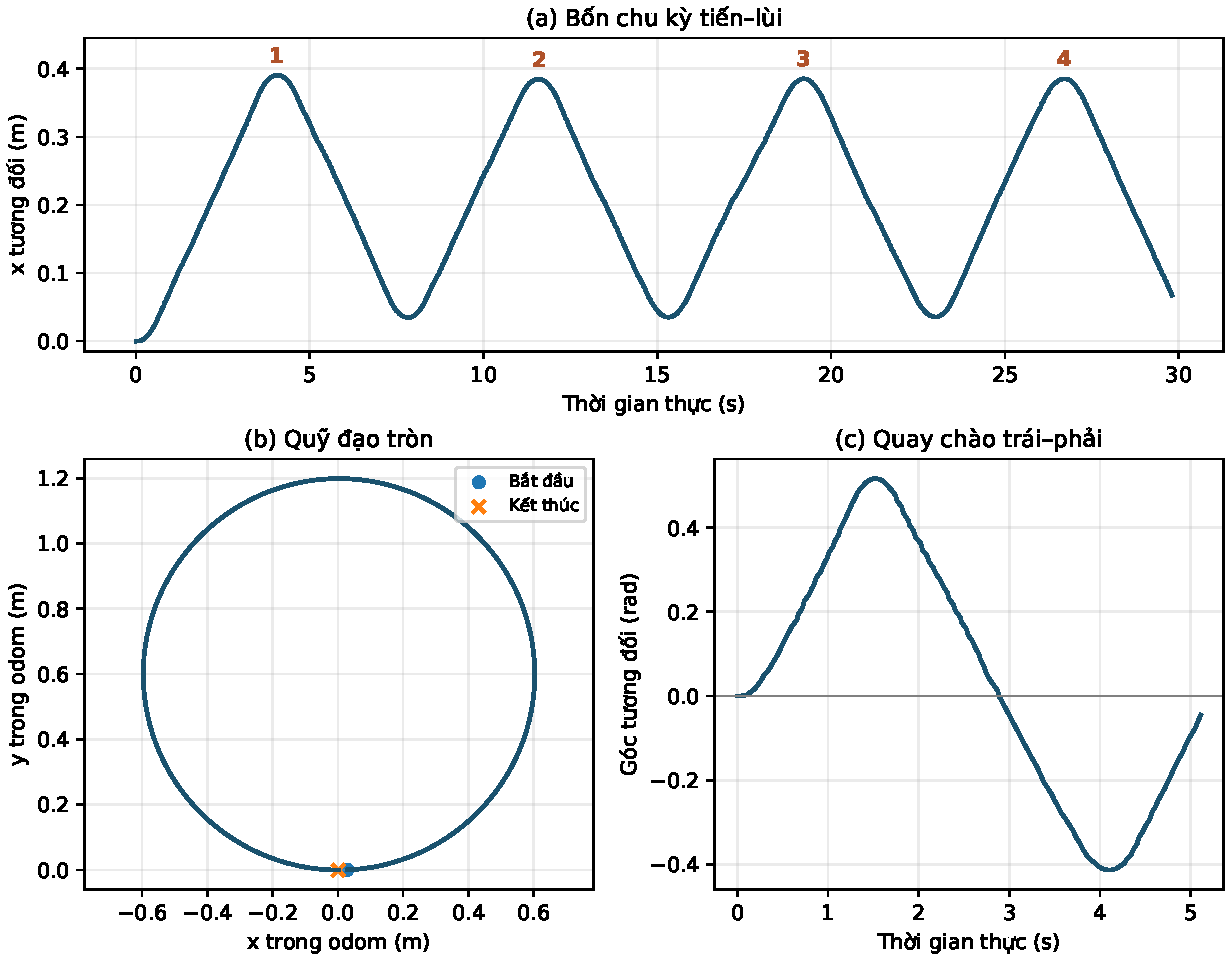
\includegraphics[width=0.98\linewidth]{images/motion_overview.pdf}
\caption{Tổng quan chuyển động từ odometry thật: bốn chu kỳ tiến--lùi, một vòng tròn và ba pha chào. Trục thời gian là đồng hồ thực.}
\label{fig:motion-overview}
\end{figure}

\begin{table}[!htbp]\centering\smalltable
\begin{tabularx}{\linewidth}{@{}p{2.4cm}p{2.0cm}LL@{}}\toprule
\textbf{Hành vi} & \textbf{Thời gian thực} & \textbf{Quan sát đo được} & \textbf{Nhận xét}\\\midrule
Tiến--lùi & 29,85 s & Bốn đỉnh; tám pha; đỉnh đầu khoảng 0,390 m. & Có vượt ngưỡng pha 0,35 m.\\
Vòng tròn & 35,70 s & Bán kính khớp khoảng 0,600 m; độ khép kín khoảng 0,028 m. & Đánh giá trong odom, chưa so với ground truth.\\
Chào & 5,15 s & Góc tương đối từ khoảng $+0,516$ đến $-0,414$ rad; cuối $-0,045$ rad. & Đúng thứ tự, còn lệch góc.\\\bottomrule
\end{tabularx}
\caption{Phân tích ngắn theo dữ liệu của từng hành vi, không suy từ ảnh đứng.}
\end{table}

Độ vượt ở pha tiến/quay phản ánh giới hạn của điều khiển tiến độ hiện tại: chưa dùng sai số vị trí có dấu và giảm tốc theo khoảng còn lại. Thời gian thực cũng không so trực tiếp với thời gian lý tưởng mô phỏng vì còn tăng/giảm tốc và real-time factor.

\subsection{Dừng, hủy và mất tín hiệu}

\begin{figure}[!htbp]\centering
\begin{subfigure}{0.32\linewidth}\centering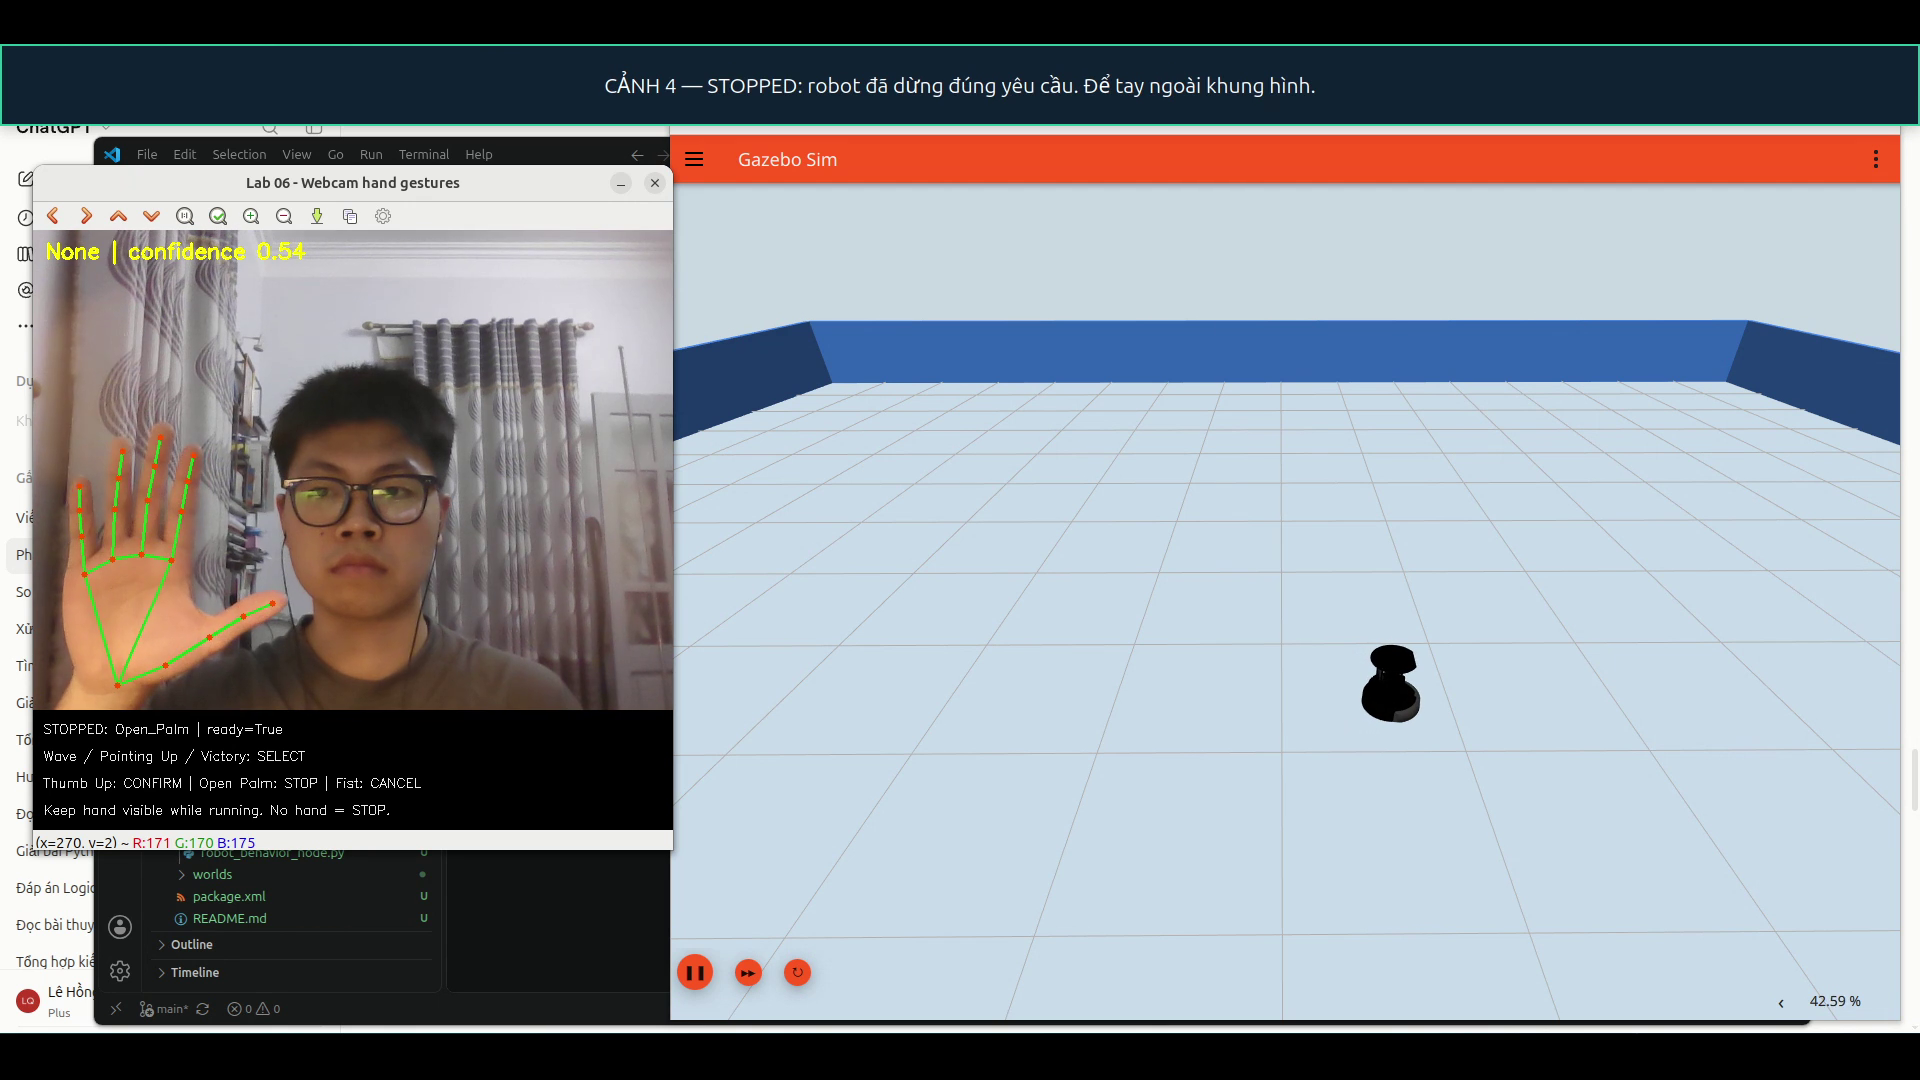
\includegraphics[width=\linewidth,trim=33bp 250bp 1247bp 230bp,clip]{images/09_open_palm_stopped.png}\caption{STOPPED}\end{subfigure}\hfill
\begin{subfigure}{0.32\linewidth}\centering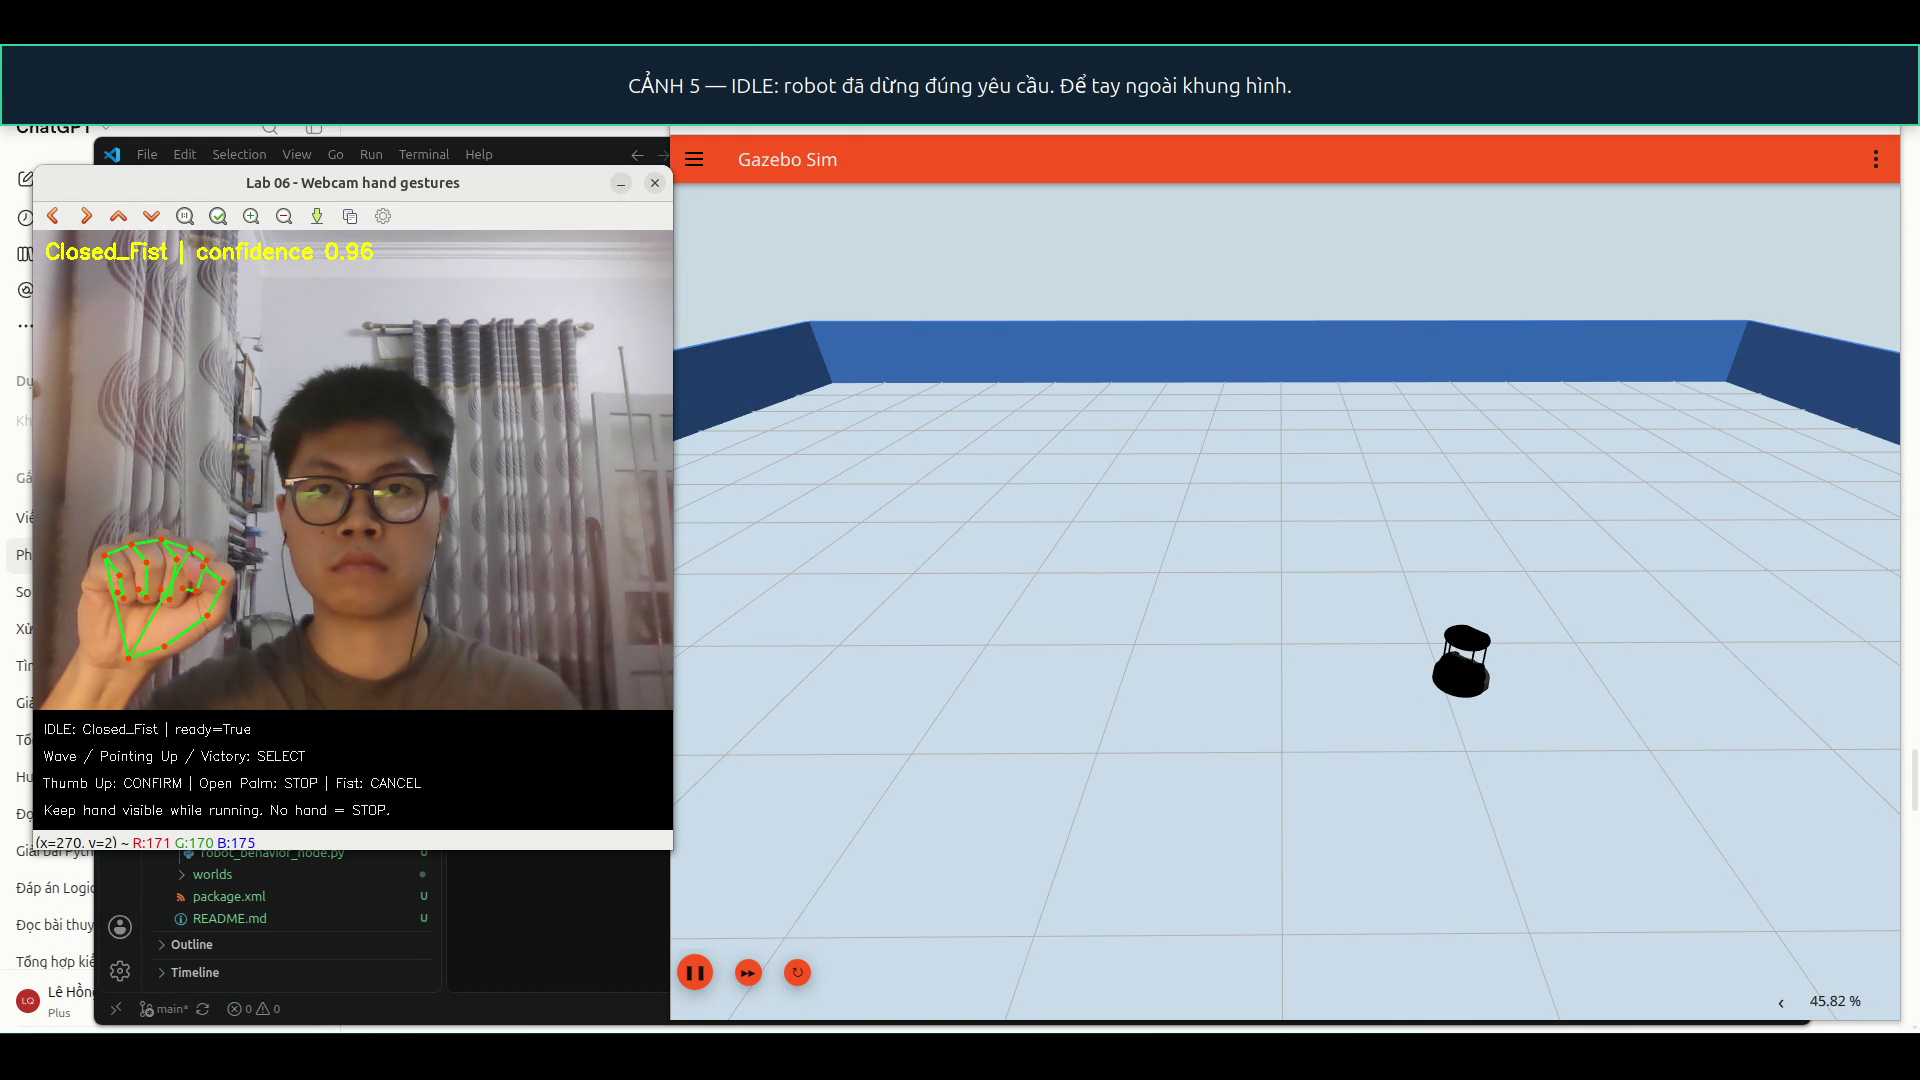
\includegraphics[width=\linewidth,trim=33bp 250bp 1247bp 230bp,clip]{images/10_closed_fist_idle.png}\caption{IDLE}\end{subfigure}\hfill
\begin{subfigure}{0.32\linewidth}\centering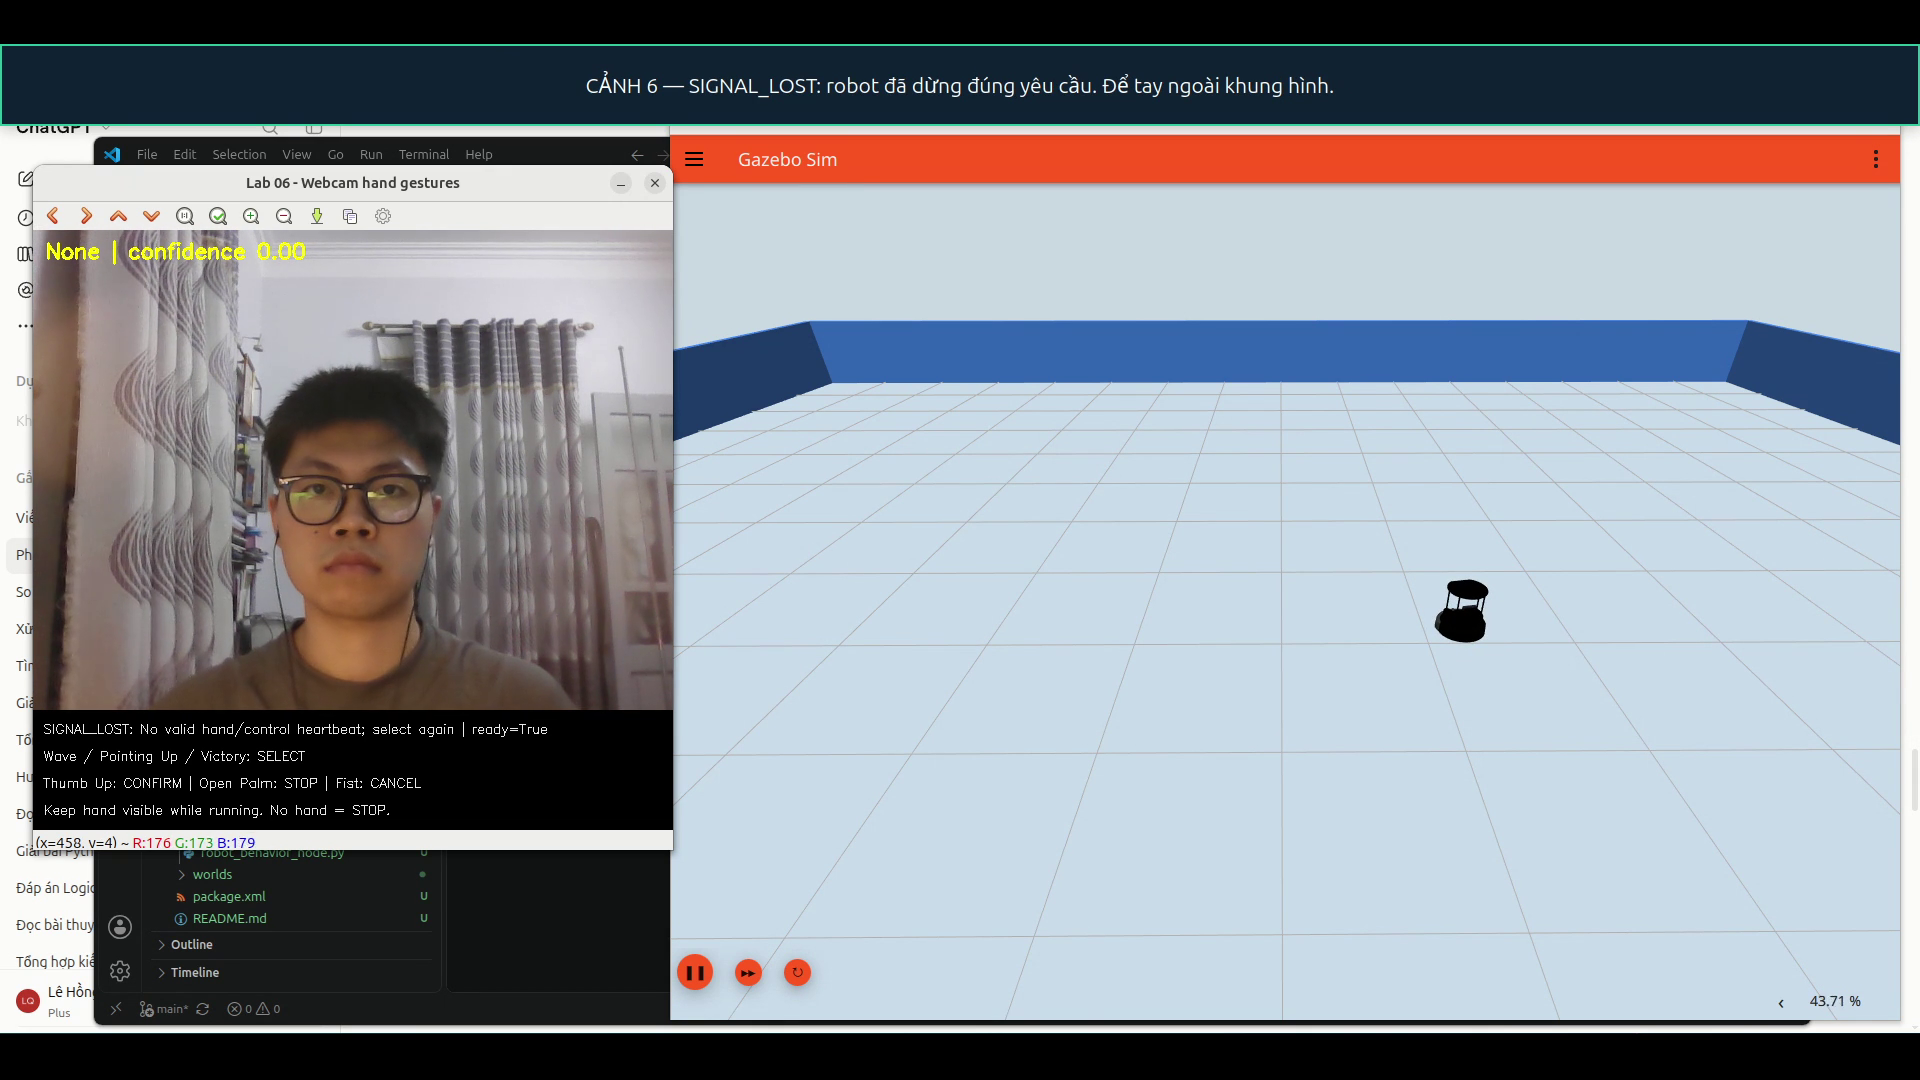
\includegraphics[width=\linewidth,trim=33bp 250bp 1247bp 230bp,clip]{images/11_signal_lost.png}\caption{SIGNAL\_LOST}\end{subfigure}
\caption{Cắt đúng vùng webcam/trạng thái từ ảnh ghi màn hình. Trong ảnh STOPPED, nhãn hiện tại đã dao động về None; lý do dừng lưu lại là Open Palm.}
\label{fig:stops}
\end{figure}

\begin{table}[!htbp]\centering\smalltable
\begin{tabularx}{\linewidth}{@{}p{1.1cm}Lp{3cm}p{2.1cm}p{1.9cm}@{}}\toprule
\textbf{Cảnh} & \textbf{Nội dung} & \textbf{Trạng thái đạt} & \textbf{Mốc đạt (s)} & \textbf{Thử lại}\\\midrule
1 & Bốn chu kỳ tiến--lùi & \code{COMPLETED} & 47,22 & 0\\
2 & Một vòng tròn & \code{COMPLETED} & 92,87 & 0\\
3 & Chào sau Wave & \code{COMPLETED} & 115,22 & 1\\
4 & Open Palm khi đang chạy & \code{STOPPED} & 144,57 & 1\\
5 & Closed Fist khi đang chạy & \code{IDLE} & 157,68 & 0\\
6 & Đưa tay khỏi webcam & \code{SIGNAL_LOST} & 171,52 & 0\\\bottomrule
\end{tabularx}
\caption{Sáu cảnh đạt sau thao tác; mốc đạt xấp xỉ trong lượt ghi. Thử lại là số đoạn gián đoạn, không phải số lỗi phân loại theo frame.}
\label{tab:results}
\end{table}

\subsection{Vấn đề thực tế và cách xử lý}

\begin{table}[!htbp]\centering\smalltable
\begin{tabularx}{\linewidth}{@{}p{3cm}LL@{}}\toprule
\textbf{Hiện tượng} & \textbf{Nguyên nhân / quan sát} & \textbf{Cách xử lý}\\\midrule
Vẫy vẫn ra Open Palm & Cấu hình cũ đòi ba đảo chiều/1,8 s; đặc trưng gần cổ tay dịch chuyển ít. & Theo dõi đầu ngón; hai đảo chiều/3 s; xóa lịch sử khi đứng yên.\\
Mất tín hiệu khi đổi tư thế & Khoảng None kéo dài quá 0,65 s; đã xảy ra ở cảnh 4. & Làm lại, mở tay dứt khoát trong khung; giữ nguyên cơ chế dừng.\\
NOT\_READY & Gazebo domain 74, các node domain 76; thiếu sensor ở controller. & Đồng bộ ba terminal về domain 76; kiểm tra topic.\\
GUI thoát mã 139 & Log Qt/Ogre2 có lỗi render; chưa xác định chính xác lỗi C++. & GUI Ogre1, server/sensor Ogre2; có launch mở lại GUI~\cite{gz}.\\\bottomrule
\end{tabularx}
\caption{Tổng hợp sự cố, bằng chứng và biện pháp đã áp dụng.}
\end{table}

Ở cảnh 3, một lần lựa chọn Wave bị xóa khi tay trở về Open Palm trước xác nhận. Ở cảnh 4, một lần dừng do SIGNAL\_LOST xảy ra trước khi nhận bàn tay mở. Video giữ cả hai đoạn; sau đó các cảnh được làm lại và đạt trạng thái đích.

\subsection{Giới hạn kết luận}
\begin{itemize}
\item Một người, một video chưa đủ để tính accuracy hay ma trận nhầm lẫn. Confidence mẫu không phải tỷ lệ đúng của hệ thống.
\item 18 test tự động kiểm chứng logic xác nhận, chống lặp, dừng, Wave, tiến độ và launch; chúng không thay thế đánh giá nhận diện bằng tay thật.
\item Video 20 fps, publish 10 Hz, giới hạn capture 15 fps là các đại lượng khác nhau. 884 ảnh preview không phải tổng frame video hoặc lượt suy luận.
\item Chưa đo độ trễ dừng đầu--cuối, chưa so odom với ground truth và chưa thử vật cản động. Video chưa có cảnh riêng giơ Thumb Up sau dừng/mất tín hiệu để kiểm tra không tự chạy lại.
\end{itemize}

\section{Kết luận và hướng phát triển}
\subsection{Kết quả đạt được}
Hệ thống đã nhận sáu cử chỉ, giao tiếp qua ROS~2, chỉ thực hiện hành vi sau xác nhận và minh chứng ba chuyển động cùng dừng/hủy/mất tín hiệu. Các sơ đồ mô tả đúng luồng triển khai; ảnh và odometry của lượt quay là cơ sở đánh giá, gồm cả hai đoạn phải thao tác lại.
\subsection{Hướng cải tiến}
\begin{itemize}
\item Thu nhiều lượt có nhãn độc lập để đo nhận đúng, bỏ sót và nhầm lớp theo điều kiện ảnh.
\item Chuẩn hóa Wave theo kích thước bàn tay; đánh giá đồng thời confidence, thời gian ổn định và timeout.
\item Điều khiển theo độ dịch chuyển có dấu, giảm tốc gần đích; đo tư thế sau khi dừng ổn định.
\item Ghi đồng bộ cử chỉ--lệnh--vận tốc để đo trễ; bổ sung cảnh không tự chạy lại sau dừng/mất tín hiệu.
\end{itemize}

\begin{thebibliography}{9}\small\setlength{\itemsep}{3pt}
\addcontentsline{toc}{section}{Tài liệu tham khảo}
\bibitem{mp_overview} Google AI Edge, \emph{Gesture recognition task guide}. \url{https://developers.google.com/edge/mediapipe/solutions/vision/gesture_recognizer}. Truy cập 24/10/2026.
\bibitem{mp_python} Google AI Edge, \emph{Gesture recognition guide for Python}. \url{https://developers.google.com/edge/mediapipe/solutions/vision/gesture_recognizer/python}. Truy cập 24/10/2026.
\bibitem{opencv} OpenCV, \emph{Getting Started with Videos}. \url{https://docs.opencv.org/4.x/dd/d43/tutorial_py_video_display.html}. Truy cập 24/10/2026.
\bibitem{ros_topics} Open Robotics, \emph{Understanding topics}, ROS~2 Jazzy documentation (bản nguồn). \url{https://github.com/ros2/ros2_documentation/blob/jazzy/source/Tutorials/Beginner-CLI-Tools/Understanding-ROS2-Topics/Understanding-ROS2-Topics.rst}. Truy cập 24/10/2026.
\bibitem{twist} ROS~2 Common Interfaces, \emph{TwistStamped message}, nhánh Jazzy. \url{https://github.com/ros2/common_interfaces/blob/jazzy/geometry_msgs/msg/TwistStamped.msg}. Truy cập 24/10/2026.
\bibitem{tb4} TurtleBot~4 User Manual, \emph{TurtleBot 4 Simulator}. \url{https://turtlebot.github.io/turtlebot4-user-manual/software/turtlebot4_simulator.html}. Truy cập 24/10/2026.
\bibitem{gz} Gazebo, \emph{Troubleshooting -- Harmonic}. \url{https://gazebosim.org/docs/harmonic/troubleshooting/}. Truy cập 24/10/2026.
\bibitem{source} Mã nguồn thực hiện bài thực hành, package \path{src/turtlebot4_gesture_control}; cấu hình \path{config/behavior.yaml} và các node được đối chiếu khi viết báo cáo.
\bibitem{experiment} Bộ dữ liệu thực nghiệm 24/10/2026: video \path{demo_turtlebot4_gestures.mp4}, \path{events.jsonl}, \path{odometry.jsonl}, \path{results.csv} và ảnh minh chứng trong thư mục lượt quay.
\end{thebibliography}

\appendix
\section*{Phụ lục: Bộ minh chứng thực nghiệm}
\addcontentsline{toc}{section}{Phụ lục: Bộ minh chứng thực nghiệm}
Bộ minh chứng gồm video MP4 180,05 giây, ảnh webcam và trạng thái, \path{events.jsonl}, \path{odometry.jsonl}, \path{results.csv}. Các file được lưu trong lượt quay ngày 24/10/2026 và gói \path{lab06_demo_2026-10-24.zip}. Hướng dẫn biên dịch pdfLaTeX và thay thông tin bìa nằm trong README của gói mã nguồn báo cáo.

\end{document}
